\documentclass[a4paper,12pt]{article}

\usepackage{a4wide}
\usepackage{amsfonts}
\usepackage{amsmath}
\usepackage{amssymb}
\usepackage{lipsum}

\usepackage{graphicx}  % For including images

\usepackage{xcolor}  % For a colorfull presentation
\usepackage{listings}  % For presenting code 

\usepackage{hyperref}

% Definition of a style for code, matter of taste
\lstdefinestyle{mystyle}{
  language=Python,
  basicstyle=\ttfamily\footnotesize,
  backgroundcolor=\color[HTML]{F7F7F7},
  rulecolor=\color[HTML]{EEEEEE},
  identifierstyle=\color[HTML]{24292E},
  emphstyle=\color[HTML]{005CC5},
  keywordstyle=\color[HTML]{D73A49},
  commentstyle=\color[HTML]{6A737D},
  stringstyle=\color[HTML]{032F62},
  emph={@property,self,range,True,False},
  morekeywords={super,with,as,lambda},
  literate=%
    {+}{{{\color[HTML]{D73A49}+}}}1
    {-}{{{\color[HTML]{D73A49}-}}}1
    {*}{{{\color[HTML]{D73A49}*}}}1
    {/}{{{\color[HTML]{D73A49}/}}}1
    {=}{{{\color[HTML]{D73A49}=}}}1
    {/=}{{{\color[HTML]{D73A49}=}}}1,
  breakatwhitespace=false,
  breaklines=true,
  captionpos=b,
  keepspaces=true,
  numbers=none,
  showspaces=false,
  showstringspaces=false,
  showtabs=false,
  tabsize=4,
  frame=single,
}
\lstset{style=mystyle}

\begin{document}
\title{Machine Learning A (2023)\\Home Assignment 3}
\author{\color{red}Niels Moctezuma Krarup, student ID: WTG176}
\date{}
\maketitle

% Please leave the table of contents as is, for the ease of navigation for TAs
\tableofcontents % Generates the table of contents
\newpage % Start a new page after the table of contents

\section{Experiment design (20 points)}
\subsection*{1)}
We have data on the form $(X_i, y_i), i = 1,\dots,2000$. $y_i \in \{0,1\}$ hence it is a classifier problem. Since we have 20 teams giving their own prediction rule we will denote these $h_n, n = 1,\dots,20$.
Each prediction rule then has an associated (unknown) expected prediction error:
$$
\mathbb{E}l(h_n(X), Y) = \mu_n, n = 1,\dots,20
$$

Which we estimate by the empirical loss:
$$
\hat{L}_n = \frac{1}{K}\sum_{i = 1}^Kl(h_n(X_i, Y_i) 
$$
Where $K$ is the number of samples set aside to evaluate the prediction rule.


Let's start by ignoring the case of selection bias for intuition sake. For simplicity let's assume only one teams is invited.

Now, since the empirical mean fulfils the assumptions for using the Hoefding bound THM 2.3 in YS, we get:
$$
\mathbb{P}(\mu_1 - \hat{L}_1 \geq 0.05) \leq -e^{2K0.05^2} 
$$
Since we want the event of underestimating by 0.05 or more, we solve the rhs to equal 0.05 and take the ceiling since we can only have whole number observations. $K =\lceil \frac{\log0.05}{-2\cdot 0.05^2} \rceil= 600$. Hence to evaluate the predictions according to the boss' wish we would need to set aside 400 subjects for training and 600 for validation/testing.

Now, since we actually have 20 teams submitting prediction rules $h(X)$ of course the smallest of the empirical losses, $\hat{L}$ will be small in virtue of being a good predictor (hopefully) but also by having a favourable (random) outcome on the validation data. 

Use use THM 3.2 with $M=20, \delta = 0.05$ and solve the error term to equal 0.05 for $K$ i.e.
$$
\sqrt{\frac{\log\frac{20}{0.05}}{2*K}} = 0.05 \Leftrightarrow \lceil K \rceil = 1199 
$$


to do a sanity check we simulate the situation with 20 teams who all give $h$ with $L(h) = 0.5$, it seems from simulations that we get a much lower necessary K, seen below:

% Placeholder figure
\begin{figure}[htbp]
    \centering
    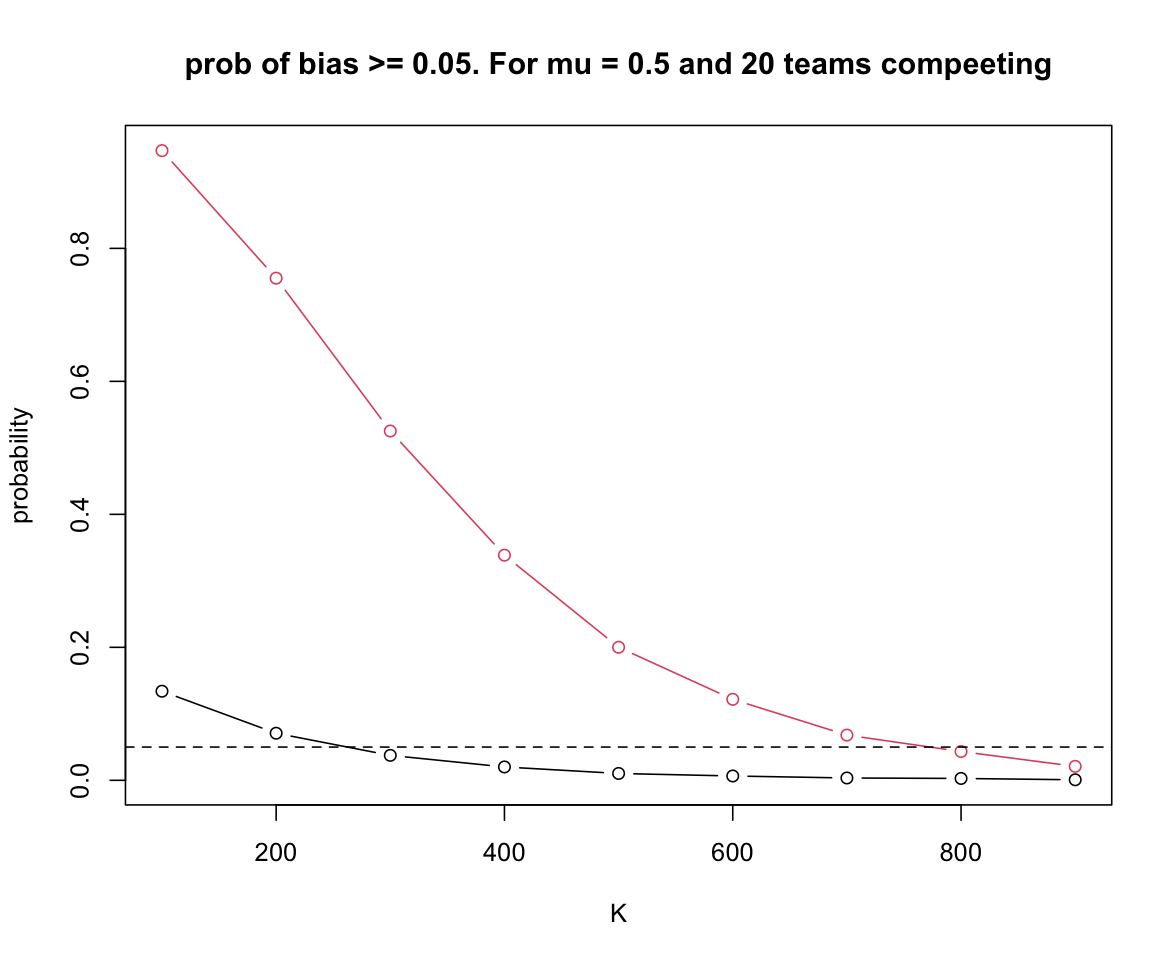
\includegraphics[width=0.5\linewidth]{1_1_b.png}
    \caption{Probability of bias given K. 20 teams (red) and 1 team (black)} % Dummy caption generated using lipsum
    \label{fig:2}
\end{figure}

\newpage

\subsection*{2)}
we now change the perspective and have a fixed training set of $n = 2000$ and validation set of $K = 1000$.
From THM 2.3 we simply fix $\delta = 0.05, K = 1000$ and solve for $M$ where we take floor since rounding up would break the inequality.
$$
\sqrt{\frac{\log\frac{M}{0.05}}{2*1000}} = 0.05 \Leftrightarrow \lfloor M \rfloor = 7 
$$
Hence we are able to accept 7 teams with the new data to fulfil the bias bound.

\section{Efficient use of the data (20 points)}
We have $2M$ models where the first $M$ models are trained on $S_0$ and validated on $S_1$ yielding empirical loss $\hat{L}(h_{0,i}, S_1), i = 1,\dots,M$ and $M$ models trained on $S_1$ and validated on $S_0$ yielding empirical loss $\hat{L}(h_{1,i}, S_0), i = 1,\dots,M$. Since the total size of the data $S = S_0 \cup S_1$ is of size $n$ and the split is even $S_0$ and $S_1$ are both of size $n/2$ observations.

We wish to derive a bound for the selected model's loss, i.e. 

$$
\mathbb{P}(L(h_{j*,i*}) - \hat{L}(h_{j*,i*}(S_{1-j*}) \leq \epsilon) \geq 1-\delta
$$

By splitting this up into the event of all $2M$ models having less bias than $\epsilon$ and taking the union probability bound we end up with 


\begin{align*}
&\mathbb{P}(L(h_{j*,i*}) - \hat{L}(h_{j*,i*}(S_{1-j*}) \geq \epsilon)  \leq \\
&\mathbb{P}(\exists m,n : L(h_{m,n}) - \hat{L}(h_{m,n}(S_{1-m}) \geq \epsilon) \leq \\
& \sum_{m,n} \mathbb{P}(L(h_{m,n}) - \hat{L}(h_{m,n}(S_{1-m}) \geq \epsilon) \leq
\underbrace{2Me^{-2n\epsilon^2}}_{\delta}
\end{align*}

Where the first equality follows from the fact that the selected prediction rule being bias greater than $\epsilon$ is a subset of the event of any $h$ having this bias.
Second follows from union bound of probability of union of events. Third is Hoefding applied on the $2M$ models.\\
finally we solve $\delta = 2Me^{-2n\epsilon^2}$ and get 
$\epsilon = 
\sqrt{ 
	\frac{\log\frac{2M}{\delta}}{2n}
	}
$
Inserting this we get a $1-\delta$ bound for the bias i.e.

$$
\mathbb{P}\left(L(h_{j*,i*}) - \hat{L}(h_{j*,i*}(S_{1-j*}) \leq \sqrt{ \frac{\log\frac{2M}{\delta}}{2n}}\right) \geq 1-\delta
$$



\section{How to split a sample into training and test sets (30 points)}
The situation is now that we have one set of data but train and evaluate the different partitions of data. The $m$ tests splits are of size $n_1,\dots,n_m$, hence the simultaneous bound for $L(\hat{h}_i)$ by splitting up the events:
\begin{align*}
&\mathbb{P}(\forall i: L(h_i) - \hat{L}(h_i) \leq \epsilon )  = \\
&\mathbb{P} (\exists i: L(h_i) - \hat{L}(h_i) \geq \epsilon)  \leq \\
&\sum_m \mathbb{P} ( L(h_m) - \hat{L}(h_m) \geq \epsilon)  \leq \\
&\sum_m e^{-2n_m\epsilon^2}
\end{align*}

This is not really nice to invert. One could bound further by using the largest $n_m$. 



\section{Preprocessing (30 points)}

\subsection{9.1 (6 points)}
Lets use the neightest neighbour algorithm on the data point $p_{unkown} = (21, 36)$
using the euclidian distance $d(x,x') = \sqrt{(x_1 - x_1')^2 + \cdots + (x_n - x_n')^2}$. we calculate the distance to the two other points $p_{good} = (47, 35), p_{bad} = (22, 40)$

\begin{lstlisting}
import numpy as np

mr_good = np.array([47, 35])
mr_bad = np.array([22, 40])
mr_unknown = np.array([21, 36])

# Calculate the Euclidean distance
def distance_scale(c, v1, v2):

  tmp_v1 = v1
  tmp_v2 = v2


  tmp_v1[1] = c*v1[1] #scale money /2nd coordinate
  tmp_v2[1] = c*v2[1] #scale money /2nd coordinate
  
  distance = np.linalg.norm(tmp_v1 - tmp_v2)

  return(distance)

# Print the result
print(
    distance_scale(1, mr_bad,  mr_unknown),
    distance_scale(1, mr_good, mr_unknown)
    )
print(
    distance_scale(10**3, mr_bad,  mr_unknown),
    distance_scale(10**3, mr_good, mr_unknown)
    )
\end{lstlisting}

we get
\begin{lstlisting}
4.123105625617661 26.019223662515376
4000.000124999998 35965000.000009395
\end{lstlisting}

i.e. in the first case Mr Unkown is closest to Mr Bad, and in the second case he is closer to Mr Good. Due to Money now being scaled up, it is weighing much more and hence the small difference in Income to Mr Good is 'weighted' higher.



\subsection{9.2 (6 points)}
By direct calculation we get
$$
\gamma X = (I - \frac{1}{N}11^T)X = X- \frac{1}{N}11^TX
$$
Note that all (i,1)-entries of the second matrix, $\frac{1}{N}11^TX$, is exeactly the sum of feature 1: $\sum_{n = 1}^N X_{n,1}$, while all the (i,2)-elements is the sum of feature 2: $\sum_{n = 1}^N X_{n,2}$. When this is multiplied by the scala $\frac{1}{N}$ we get the mean of each feature in $N$ identical rows, such that when we substract it from $X$ we center the data.

\subsection{9.4 (18 points)}
a)
Using standard rules for variance and covariance we get:
\begin{align}
&Var(x_1) = 1 \nonumber  \\
&Var(x_2) = (1-\epsilon^2)Var(\hat{x}_1) + \epsilon^2Var(\hat{x}_2) = (1-\epsilon^2) + \epsilon^2 = 1 \nonumber  \\
&Cov(x_1, x_2) = Cov(\hat{x}_1, \sqrt{(1-\epsilon^2)}\hat{x}_1 + \epsilon\hat{x}_2)  =  \nonumber  \\
&Cov(\hat{x}_1, \hat{x}_1) \sqrt{1-\epsilon^2} + Cov(\hat{x}_1, \epsilon \hat{x}_2) = \nonumber  \\
&\sqrt{(1-\epsilon^2)} \nonumber 
\end{align}

b)
We are given $f(\hat{\bold{x}}) = \hat{w}_1 \hat{x}_1 + \hat{w}_2 \hat{x}_2$ i.e. linear in the two input variables. Let's now evaluate in the correlated input $\bold{x}$:
\begin{align*}
&f(\bold{x}) =   \hat{w}_1x_1 + \hat{w}_2 x_2  = \\
& \hat{w}_1x_1 + \hat{w}_2(\sqrt{1-\epsilon^2} \hat{x}_1 + \epsilon \hat{x}_2 ) = \\
&\underbrace{\left(\hat{w}_1 + \hat{w}_2\sqrt{1-\epsilon^2} \right)}_{w_1} \hat{x}_1 + \underbrace{ \epsilon \hat{w}_2}_{\hat{x}_2} \hat{x}_2
\end{align*}

So, evaluating in $\bold{x}$ is the same as a reweighted evaluation in $\hat{\bold{x}}$ with new weights:
$w_1 = \left(\hat{w}_1 + \hat{w}_2(\sqrt{1-\epsilon^2} \right)$ and 
$w_2 = \epsilon \hat{w}_2$\newline

c)
We now have the simple target function $f(\hat{\bold{x}}) = \hat{x}_1 + \hat{x}_2$
meaning that $\hat{w}_1  = \hat{w}_2 = 1$

If we evaluate using the correlated data $\bold{x}$ with regularization constraint $w_1^2 + w_2^2 \leq C$ then we can write the constraint in $\bold{w}$ in terms of $\hat{\bold{w}}$ as such:
\begin{align*}
w_1^2 + w_2^2 &= \hat{w}_1^2 + \hat{w}_2^2 (1-\epsilon) + 2\hat{w}_1\hat{w}_2\sqrt{1-\epsilon^2} + \epsilon^2\hat{w}_2^2 \\
&= \hat{w}_1^2 + \hat{w}_2^2 + 2\sqrt{1-\epsilon^2} \hat{w}_1\hat{w}_2 \\
&= 2+2\sqrt{1-\epsilon^2}
\end{align*}

% Placeholder figure
\begin{figure}[htbp]
    \centering
    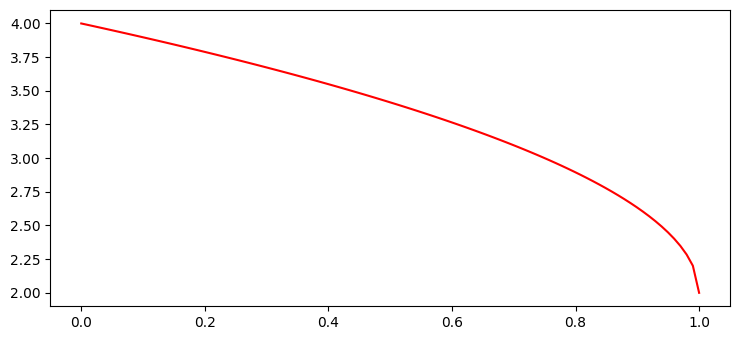
\includegraphics[width=0.5\linewidth]{4_3_a.png}
    \caption{Maximal C given epsilon} % Dummy caption generated using lipsum
    \label{fig:1}
\end{figure}



\section{Distribution of Student's Grades (Optional, 0 points)}

\bibliography{bibliography}  % If you have some references, use BibTeX

\end{document}
